\documentclass{beamer}
\usepackage{tikz}
\usepackage{graphicx} % Required for inserting images
\usepackage{amssymb}
\usepackage{amsmath}
\usepackage{soul}
\usepackage{xcolor}
\usepackage{pgfplots}
\pgfplotsset{compat=1.18}
\usetikzlibrary{positioning}


\usecolortheme{orchid}

\title{Phragmén–Lindelöf e o princípio de incerteza de Hardy}
\author{Afonso Vilhena Francisco }
\date{21 Março 2026, Fundação Calouste Gulbenkian}

\begin{document}

\begin{frame}{}
    \titlepage
    $$\textbf{Tutor: } \text{Diogo Oliveira e Silva}$$

\end{frame}


\begin{frame}{}

\begin{block}{Princípio do Módulo Máximo}
Sejam $A$ uma região conexa e limitada e $f:\overline{A} \rightarrow \mathbb{C}$ contínua e holomorfa em $A$. 

Então, $$|f(z)| \leq \max_{z_0 \in \partial A}|f(z_0)|, \text{ para qualquer } z \in A$$
\end{block}\\

\vspace{1cm}

\begin{columns}
    \begin{column}{0.48\textwidth}
    \centering
    \begin{tikzpicture}[scale=0.7]
    \begin{axis}[
        axis lines = middle,
        xmin=0, xmax=pi,
        ymin=0.5, ymax=1.01,
        %xtick = {pi/4, pi/2, 3*pi/4},
        %xticklabels = {$\frac{\pi}{4}$, $\frac{\pi}{2}$, $\frac{3\pi}{4}$},
        %ytick = {0,1/2,1},
        xlabel = $x$,
        ylabel = $y$,
        domain = pi/4:3*pi/4,
        samples = 200,
    ]
    \addplot[thick, smooth] {sin(deg(x))};
    \end{axis}
    \end{tikzpicture}
    \end{column}

    \begin{column}{0.48\textwidth}
        \centering
        
\includegraphics[width=0.6\linewidth]{Maximum_modulus_principle.png}
    \end{column}
\end{columns}

\end{frame}


\begin{frame}{}

\begin{columns}[T]

\column{0.68\textwidth}

\underline{\textbf{Exemplo:}} Considere-se a função $f(z)=e^{-iz}$ e $A=[0,1]\times[0,1]$.
$$|f(z)|=|e^{-i(x+iy)}|=e^{y}$$
que toma o máximo para $y=1$ e $0\le x\le 1$.

\vspace{1.5cm}

Considere-se agora $A=\{z\in\mathbb{C}\mid \Im(z)>0\}$.
Para $z\in\partial{A},\; z=x\in\mathbb{R}$.
$$|f(z)|=|e^{-ix}|=1$$
Mas$$|f(2i)|=|e^{-i\,2i}|=e^2>1.$$


\column{0.4\textwidth}

\centering

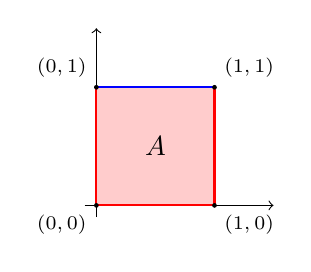
\begin{tikzpicture}[scale=1.5]

\draw[->] (-0.1,0) -- (1.5,0);
\draw[->] (0,-0.1) -- (0,1.5);

\fill[red!20] (0,0) rectangle (1,1);
\draw[red, thick] (0,0) rectangle (0,1);
\draw[red, thick] (0,0) rectangle (1,0);
\draw[red, thick] (1,0) rectangle (1,1);
\draw[blue, thick] (0,1) rectangle (1,1);

\fill (0,0) circle (0.02);
\fill (1,0) circle (0.02);
\fill (0,1) circle (0.02);
\fill (1,1) circle (0.02);

\node[below left, font=\scriptsize] at (0,0) {$(0,0)$};
\node[below right, font=\scriptsize] at (1,0) {$(1,0)$};
\node[above left, font=\scriptsize] at (0,1) {$(0,1)$};
\node[above right, font=\scriptsize] at (1,1) {$(1,1)$};

\node at (0.5,0.5) {$A$};

\end{tikzpicture}

\vspace{2cm}

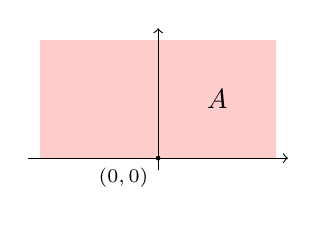
\begin{tikzpicture}[scale=1.5]

\fill[red!20] (-1,0) rectangle (1,1);

\draw[red, dashed] (-1,0) -- (1,0);

\draw[->] (-1.1,0) -- (1.1,0);
\draw[->] (0,-0.1) -- (0,1.1);

\fill (0,0) circle (0.02);
\node[below left, font=\scriptsize] at (0,0) {$(0,0)$};

\node at (0.5,0.5) {$A$};

\end{tikzpicture}

\end{columns}

\end{frame}



\begin{frame}{}

\begin{block}{Princípio de Phragmén–Lindelöf}
Sejam $A$ um setor circular de ângulo $\pi / \beta$ e $f:\overline{A} \rightarrow \mathbb{C}$ contínua e holomorfa em $A$ tal que 
\begin{itemize}
    \item \vert f(z)|  \leq 1, \text{ para todo o\;} $z \in \partial A$
    \item \vert f(z)|  $\leq Ce^{c|z|^\alpha}, \text{ para todo } z \in A \text{ e alguns } C,c>0 $
    e $0<\alpha<\beta$
\end{itemize}\\

Então, $$|f (z)| \leq 1, \;\;\;\; \text{para todo o } z \in A.$$
\end{block}

\centering
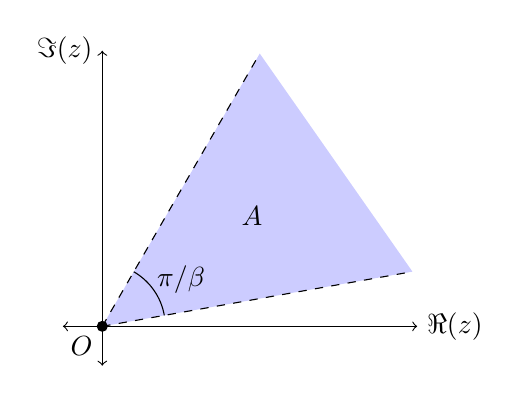
\begin{tikzpicture}
    \def\r{1}
    \def\a{10}
    \def\b{60}

    \draw[<->] (-0.5,0) -- (4,0) node[right] {$\Re(z)$};
    \draw[<->] (0,-0.5) -- (0,3.5) node[left] {$\Im(z)$};

    \fill[blue!20]
        (0,0) -- (\a:4) -- (\b:4) -- cycle;

    \draw[dashed] (0,0) -- (\a:4);
    \draw[dashed] (0,0) -- (\b:4);

    \fill (0,0) circle (2pt) node[below left] {$O$};

    \draw (\a:0.8) arc (\a:\b:0.8);
    \node at (1,0.6) {$\pi/\beta$};

    \node at (1.9,1.4) {$A$};

\end{tikzpicture}


\end{frame}


\begin{frame}{}

\begin{block}{Princípio de Phragmén–Lindelöf}
Sejam $A$ um setor circular de ângulo $\pi / \beta$ e $f:\overline{A} \rightarrow \mathbb{C}$ contínua e holomorfa em $A$ tal que 
\begin{itemize}
    \item \vert f(z)|  \leq 1, \text{ para todo o\;} $z \in \partial A$
    \item \vert f(z)|  $\leq Ce^{c|z|^\alpha}, \text{ para todo } z \in A \text{ e alguns } C,c>0 $
    e $0<\alpha<\beta$
\end{itemize}\\

Então, $$|f (z)| \leq 1, \;\;\;\; \text{para todo o } z \in A.$$
\end{block}


\underline{\textbf{Exemplo anterior:}}

\vspace{0.2cm}

$f(z)=e^{-iz} \text { e } A=\{z \in \mathbb{C}\mid \Im{(z)} >0 \}$.

Seja $z=Ri$, $R>0$ então $$e^R=|f(z)| \leq Ce^{cR^\alpha} \Leftrightarrow e^{R-cR^\alpha} \leq  C \xrightarrow{R \to \infty} \infty \leq C$$

\end{frame}



\begin{frame}{}
    \begin{block} {Princípio de Incerteza de Hardy}
        Seja $f: \mathbb{R} \rightarrow \mathbb{C}$ tal que $f(x)=O(e^{-\pi Ax^2 })$ e $\hat{f}(\xi)=O(e^{-\pi B \xi^2})$, com $A,B >0$.
        Se:
        \begin{itemize}
            \item $AB=1$, então $f(x)=Ce^{-\pi Ax^2}$, com $C \in \mathbb{R}$
            \item $AB>1$, então $f \equiv 0$
        \end{itemize}
    \end{block}

\pause

\begin{center}
\resizebox{0.95\textwidth}{!}{
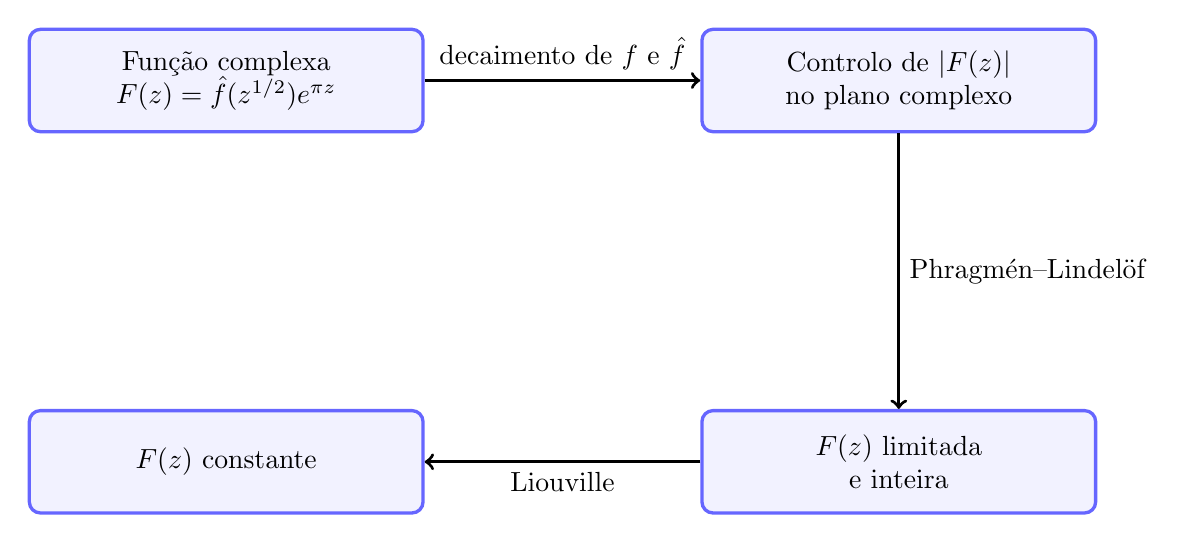
\begin{tikzpicture}[
    node distance=3.5cm,
    SIR/.style={
        rectangle, 
        draw=blue!60, 
        fill=blue!5, 
        very thick,
        rounded corners,
        minimum width=5cm,
        minimum height=1.3cm,
        align=center
    },
    arrow/.style={->, very thick}
]

\node[SIR] (A) 
{Função complexa\\ $F(z)=\hat{f}(z^{1/2})e^{\pi z}$};

\node[SIR] (B) [right=of A] 
{Controlo de $|F(z)|$\\ no plano complexo};

\node[SIR] (C) [below=of B] 
{$F(z)$ limitada\\ e inteira};

\node[SIR] (D) [below=of A] 
{$F(z)$ constante};

\draw[arrow] (A) -- node[above] {decaimento de $f$ e $\hat{f}$} (B);
\draw[arrow] (B) -- node[right] {Phragmén--Lindelöf} (C);
\draw[arrow] (C) -- node[below] {Liouville} (D);

\end{tikzpicture}
}
\end{center}
\end{frame}

\begin{frame}{Próximos Passos}
\begin{beamercolorbox}[colsep*=.75ex, rounded=true, shadow=false]{block body}
    Dada $\mathcal{C}$ coleção de funcões $f: \mathbb{R} \rightarrow \mathbb{C}$, $(A, \widehat{A}) \subset \mathbb{R}^2$ diz-se um \textbf{par único} para $\mathcal{C}$ se 
    \[
    \begin{aligned}
        f(x) &= 0 \quad \text{para todo } x \in A\\
        \hat{f}(\xi) &= 0 \quad \text{para todo } \xi \in \widehat{A}
    \end{aligned}
    \quad \Rightarrow \quad
    f \equiv 0
    \]
\end{beamercolorbox}
\vspace{0.2cm}

\pause

\textbf{Exemplo:} $f \in L^2(\mathbb{R})$, $\operatorname{supp}(\hat{f})=[-\delta/2,\delta/2] $
\vspace{-0.5cm}

$$f(x) = \sum_{k=-\infty}^\infty{f(k/\delta)\frac{\sin(\pi(\delta x-k))}{\pi(\delta x-k)}}\,, \;\;\;\;\;\;\;\;\;\;\text{ (Shannon –
Whittaker)}$$

$\therefore \left(\frac{1}{\delta}\mathbb{Z}, \mathbb{R} \backslash [-\delta/2,\delta/2]  \right)$ é um par único para $L^2 (\mathbb{R})$.
\vspace{0.6cm}

\end{frame}

\begin{frame}{Próximos Passos}
    \textbf{Questão:} Que condições em $(\alpha, \beta)$ são necessárias para que
    $$A=\{\pm n^\alpha \}_{n \in \mathbb{N}} \text{ e } \hat{A}=\{\pm n^\beta \}_{n \in \mathbb{N}}$$

    seja um par único em $\mathcal{S}(\mathbb{R}).$
\end{frame}

\end{document}
